\section*{Questão 1}

Responda as seguintes perguntas usando o dataset fornecido:

\begin{enumerate}

\item Visualize os dados (em 2 ou 3 dimensões) para entender a estrutura dos dados.
Explique o que você fez para visualizar as figuras. Descreva sua abordagem para visualizar os dados e quais insights podem ser obtidos do gráfico, se algum.

\begin{tcolorbox}[colback=white, colframe=black, title=Resposta:]
    Para visualizar os dados, utilizei a função `visualizar\_dados', que gera gráficos em 2 e 3 dimensões a partir do dataset fornecido. No código, carreguei o dataset usando a biblioteca pandas e extraí as colunas `feature 1', `feature 2' e `feature 3', além da coluna `class label'.
    
    Em seguida, criei gráficos 2D para todas as combinações de features (figuras \ref{fig:q1_i1_x1x2}, \ref{fig:q1_i1_x1x3} e \ref{fig:q1_i1_x2x3}). As combinações consideradas foram `feature 1` vs `feature 2`, `feature 1` vs `feature 3` e `feature 2` vs `feature 3`. Para cada gráfico 2D, utilizei a função `scatter` do matplotlib, onde as cores dos pontos representam as diferentes classes. Para facilitar a identificação, adicionei uma legenda correspondente a cada classe.
    
    Por fim, também plotei os dados em um gráfico 3D (figura \ref{fig:q1_i1_3d} ), representando as três features simultaneamente. Esse gráfico permite uma visualização mais abrangente da estrutura dos dados.
    
    A análise visual revela que as classes parecem estar bem separadas, principalmente no gráfico 3D, o que sugere que um modelo de mistura de gaussianas pode ser adequado para representar os dados. As classe 1 e 4, em todas as vistas, estão bem afastadas das demais classes, enquanto as classes 2 e 3 possuem uma fronteira mais tenue entre si. Existem alguns pontos de sobreposição entre as classes, mas no geral elas estão bem separadas.
\end{tcolorbox}

\begin{figure}[H]
    \centering
    \begin{subfigure}{0.45\textwidth}
        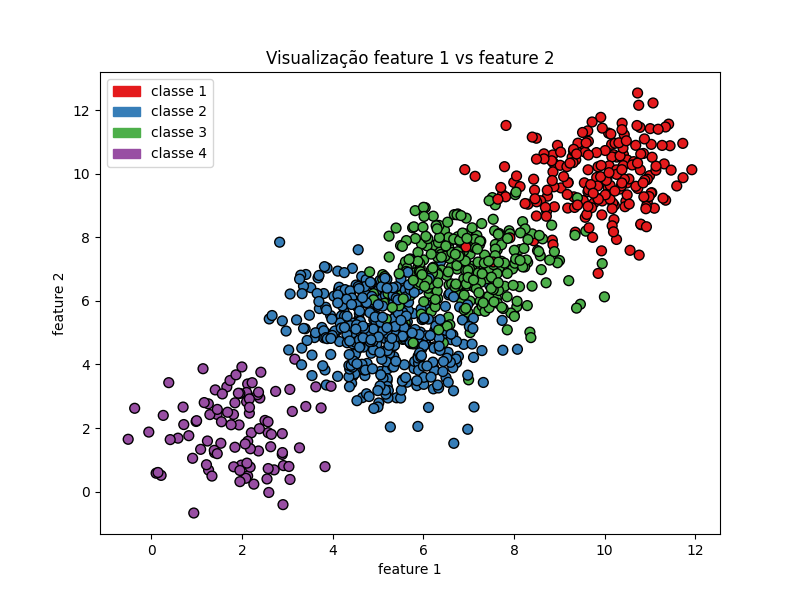
\includegraphics[width=\textwidth]{fig/q1_i1_x1x2.png}
        \caption{Feature 1 vs Feature 2}
        \label{fig:q1_i1_x1x2}
    \end{subfigure}
    \hfill
    \begin{subfigure}{0.45\textwidth}
        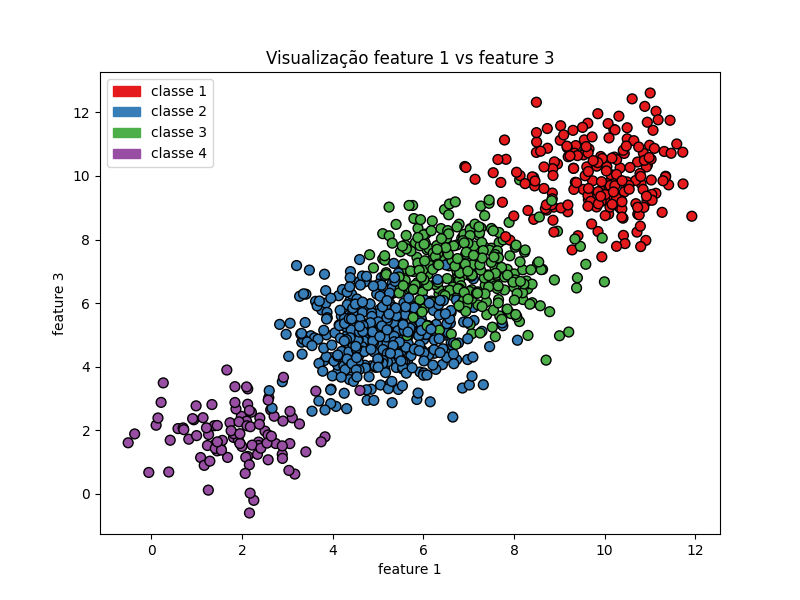
\includegraphics[width=\textwidth]{fig/q1_i1_x1x3.png}
        \caption{Feature 1 vs Feature 3}
        \label{fig:q1_i1_x1x3}
    \end{subfigure}
    
    \vspace{0.5cm}
    
    \begin{subfigure}{0.45\textwidth}
        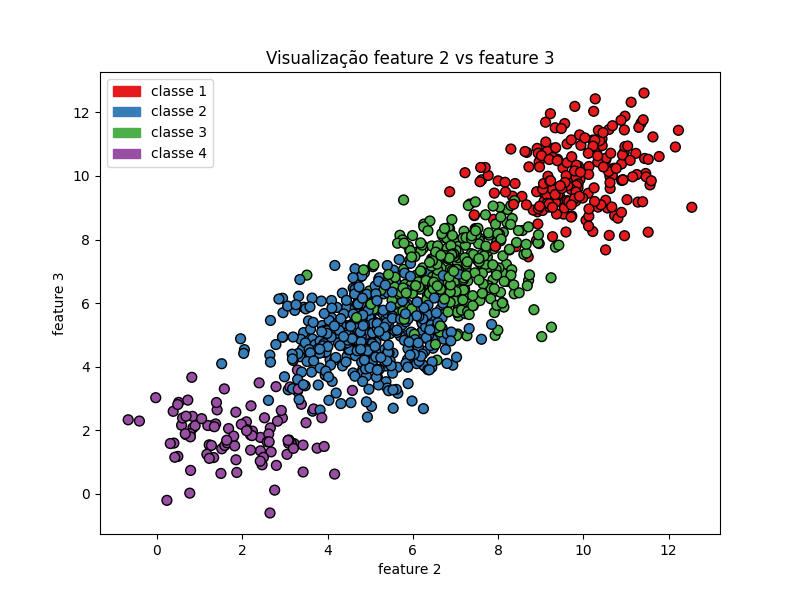
\includegraphics[width=\textwidth]{fig/q1_i1_x2x3.png}
        \caption{Feature 2 vs Feature 3}
        \label{fig:q1_i1_x2x3}
    \end{subfigure}
    \hfill
    \begin{subfigure}{0.45\textwidth}
        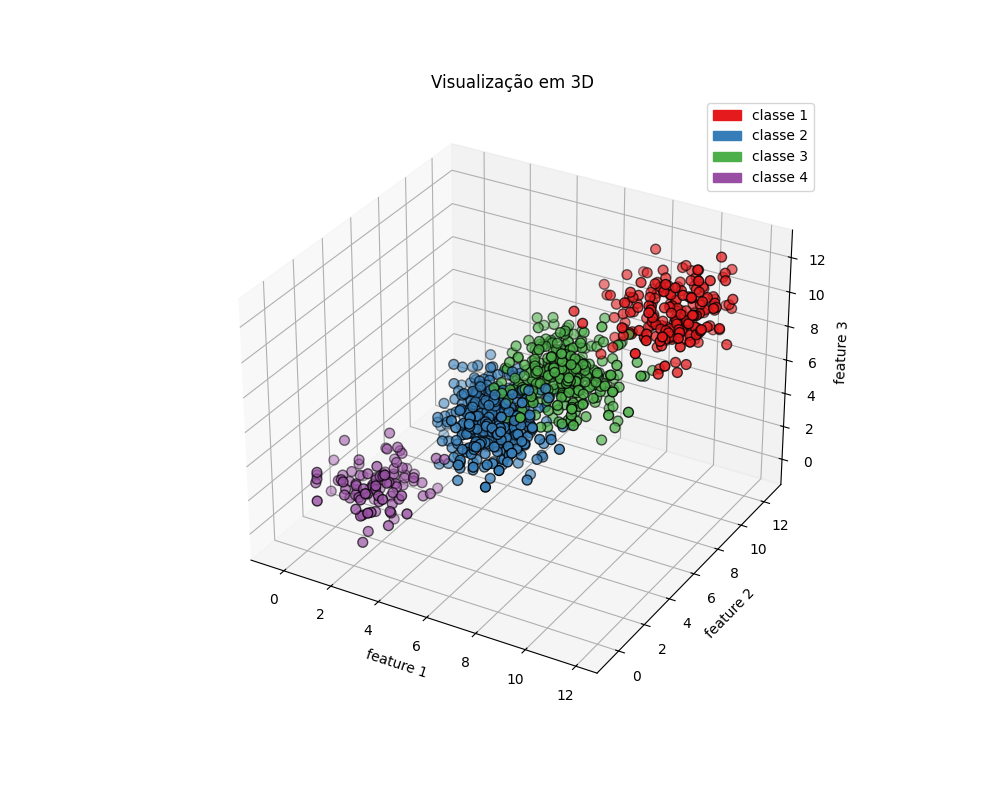
\includegraphics[width=\textwidth]{fig/q1_i1_3d.png}
        \caption{Gráfico 3D das features}
        \label{fig:q1_i1_3d}
    \end{subfigure}
    
    \caption{Visualização dos dados em 2D e 3D}
    \label{fig:q1_i1_combined}
\end{figure}

\item Ajuste uma mistura de gaussianas com 4 componentes ao conjunto de dados. Calcule TODOS os parâmetros necessários para o modelo. Explique todas as etapas. Forneça detalhes de como você determina os parâmetros de melhor ajuste para cada modelo de mistura e descreva o processo de ajuste do modelo.

\begin{tcolorbox}[colback=white, colframe=black, title=Resposta:]
    \textbf{Passos para o MLE em uma Mistura de Gaussianas com Labels Conhecidos:}

    \begin{enumerate}
        \item \textbf{Função de Verossimilhança:} \\
        Dado que temos os rótulos \( y_i \) que indicam a qual gaussiana cada ponto \( x_i \) pertence, a função de verossimilhança é dada por:
        \[
        L(\mu_k, \sigma_k^2, \pi_k) = \prod_{i=1}^{N} \prod_{k=1}^{K} \left[ \pi_k \cdot \mathcal{N}(x_i | \mu_k, \sigma_k^2) \right]^{\mathbb{1}(y_i = k)}
        \]
        Onde \( \mathbb{1}(y_i = k) \) é a função indicadora que vale 1 quando o dado \( x_i \) pertence à classe \( k \) e \( \mathcal{N}(x_i | \mu_k, \sigma_k^2) \) é a densidade da gaussiana.
    
        \item \textbf{Função de Log-Verossimilhança:} \\
        Tomamos o logaritmo da função de verossimilhança para simplificar o processo de maximização:
        \[
        \log L(\mu_k, \sigma_k^2, \pi_k) = \sum_{i=1}^{N} \sum_{k=1}^{K} \mathbb{1}(y_i = k) \left[ \log \pi_k - \frac{1}{2} \log (2\pi \sigma_k^2) - \frac{(x_i - \mu_k)^2}{2\sigma_k^2} \right]
        \]
    
        \item \textbf{Maximização via Derivação:}
        \begin{itemize}
            \item \textbf{Derivada em relação a \( \mu_k \):} \\
            A derivada da log-verossimilhança em relação a \( \mu_k \) é:
            \[
            \frac{\partial \log L}{\partial \mu_k} = \sum_{i=1}^{N} \mathbb{1}(y_i = k) \frac{(x_i - \mu_k)}{\sigma_k^2}
            \]
            Igualando a zero, obtemos a estimativa para \( \mu_k \):
            \[
            \mu_k = \frac{1}{N_k} \sum_{x_i \in X_k} x_i
            \]
            Onde \( N_k \) é o número de amostras na classe \( k \).
    
            \item \textbf{Derivada em relação a \( \sigma_k^2 \):} \\
            A derivada da log-verossimilhança em relação a \( \sigma_k^2 \) é:
            \[
            \frac{\partial \log L}{\partial \sigma_k^2} = \sum_{i=1}^{N} \mathbb{1}(y_i = k) \left( -\frac{1}{2\sigma_k^2} + \frac{(x_i - \mu_k)^2}{2\sigma_k^4} \right)
            \]
            Igualando a zero, obtemos a estimativa para \( \sigma_k^2 \):
            \[
            \sigma_k^2 = \frac{1}{N_k} \sum_{x_i \in X_k} (x_i - \mu_k)^2
            \]
        \end{itemize}
    \end{enumerate}
\end{tcolorbox}

\begin{tcolorbox}[colback=white, colframe=black, title=Resposta(continuação):]
    
    \begin{enumerate}
        \setcounter{enumii}{2}
        \item \textbf{Maximização via Derivação (cont.):}
        
        \begin{itemize}
            \item \textbf{Derivada em relação a \( \pi_k \):} \\
            Com a restrição \( \sum_{k=1}^{K} \pi_k = 1 \), derivamos a log-verossimilhança em relação a \( \pi_k \):
            \[
            \frac{\partial \log L}{\partial \pi_k} = \sum_{i=1}^{N} \frac{\mathbb{1}(y_i = k)}{\pi_k}
            \]
            Igualando a zero, obtemos a estimativa para \( \pi_k \):
            \[
            \pi_k = \frac{N_k}{N}
            \]
        \end{itemize}

    
        \item \textbf{Resumo das Soluções Fechadas:} \\
        - Médias: \( \mu_k = \frac{1}{N_k} \sum_{x_i \in X_k} x_i \) \\
        - Variâncias: \( \sigma_k^2 = \frac{1}{N_k} \sum_{x_i \in X_k} (x_i - \mu_k)^2 \) \\
        - Pesos: \( \pi_k = \frac{N_k}{N} \)
    
    \end{enumerate}
    

\textbf{Implementação:}
Utilizando um codigo python (presente no repositório no final deste relatório), as fórmulas finais para cada parâmetro foram implementadas e os resultados podem ser vistos nas tabelas \ref{tab:means}, \ref{tab:covariances}, \ref{tab:weights} e \ref{tab:log-lokelihood}.

\end{tcolorbox}

% Tabela das Médias
\begin{table}[H]
    \centering
    \caption{Médias das Gaussianas}
    \begin{tabular}{|c|c|c|c|}
        \hline
        Classe & Média 1 & Média 2 & Média 3 \\ \hline
        1 & 9.8397 & 9.8468 & 9.9668 \\ \hline
        2 & 5.1378 & 4.9909 & 5.0114 \\ \hline
        3 & 6.9380 & 7.0204 & 7.0432 \\ \hline
        4 & 1.9207 & 1.9505 & 1.9004 \\ \hline
    \end{tabular}
    \label{tab:means}
\end{table}

% Tabela das Variâncias
\begin{table}[H]
    \centering
    \caption{Variâncias das Gaussianas}
    \begin{tabular}{|c|c|c|c|}
        \hline
        Classe & Variância 1 & Variância 2 & Variância 3 \\ \hline
        1 & 1.0293 & 1.0579 & 1.0586 \\ \hline
        2 & 0.9491 & 1.1505 & 0.9616 \\ \hline
        3 & 0.9962 & 0.9633 & 0.9925 \\ \hline
        4 & 0.9186 & 1.2481 & 0.6929 \\ \hline
    \end{tabular}
    \label{tab:covariances}
\end{table}

% Tabela dos Pesos
\begin{table}[H]
    \centering
    \caption{Pesos das Gaussianas}
    \begin{tabular}{|c|c|}
        \hline
        Classe & Peso \\ \hline
        1 & 0.2 \\ \hline
        2 & 0.4 \\ \hline
        3 & 0.3 \\ \hline
        4 & 0.1 \\ \hline
    \end{tabular}
    \label{tab:weights}
\end{table}

% Tabela das Log-Verossimilhanças
\begin{table}[H]
    \centering
    \caption{Log-Verossimilhança das Gaussianas}
    \begin{tabular}{|c|c|c|c|}
        \hline
        Classe & Log-LH 1 & Log-LH 2 & Log-LH 3 \\ \hline
        1 & -492.2914 & -486.7800 & -486.6553 \\ \hline
        2 & -1002.2144 & -927.7639 & -996.4297 \\ \hline
        3 & -719.5939 & -729.7360 & -720.7003 \\ \hline
        4 & -243.2974 & -217.5307 & -279.9042 \\ \hline
    \end{tabular}
    \label{tab:log-lokelihood}
\end{table}

\item Suponha que as classes 1 e 2 sejam uma mesma classe. Ajuste uma mistura de gaussianas com 3 componentes ao conjunto de dados.

\begin{tcolorbox}[colback=white, colframe=black, title=Resposta:]
Para responder a essa pergunta, fiz as seguintes alterações no código do item anterior:
    \begin{itemize}
        \item Unificação das Classes: A classe 2 foi substituída por 1 na coluna `class label' para tratar classes 1 e 2 como uma única classe.
        \item Ajuste da Mistura de Gaussianas: A mistura de gaussianas foi ajustada utilizando 3 componentes, refletindo a unificação das classes.
    \end{itemize}
Os resultados obtidos estão nas tabelas \ref{tab:means_3}, \ref{tab:covariances_3}, \ref{tab:weights_3} e \ref{tab:log-likelihood_3}.
\end{tcolorbox}

% Tabela das Médias
\begin{table}[H]
    \centering
    \caption{Médias das Gaussianas}
    \begin{tabular}{|c|c|c|c|}
        \hline
        Classe & Média 1 & Média 2 & Média 3 \\ \hline
        1 & 6.7051 & 6.6095 & 6.6632 \\ \hline
        3 & 6.9380 & 7.0204 & 7.0432 \\ \hline
        4 & 1.9207 & 1.9505 & 1.9004 \\ \hline
    \end{tabular}
    \label{tab:means_3}
\end{table}

% Tabela das Variâncias
\begin{table}[H]
    \centering
    \caption{Variâncias das Gaussianas}
    \begin{tabular}{|c|c|c|c|}
        \hline
        Classe & Variância 1 & Variância 2 & Variância 3 \\ \hline
        1 & 5.8888 & 6.3597 & 6.4509 \\ \hline
        3 & 0.9962 & 0.9633 & 0.9925 \\ \hline
        4 & 0.9186 & 1.2481 & 0.6929 \\ \hline
    \end{tabular}
    \label{tab:covariances_3}
\end{table}

% Tabela dos Pesos
\begin{table}[H]
    \centering
    \caption{Pesos das Gaussianas}
    \begin{tabular}{|c|c|}
        \hline
        Classe & Peso \\ \hline
        1 & 0.6 \\ \hline
        3 & 0.3 \\ \hline
        4 & 0.1 \\ \hline
    \end{tabular}
    \label{tab:weights_3}
\end{table}

% Tabela das Log-Verossimilhanças
\begin{table}[H]
    \centering
    \caption{Log-Verossimilhança das Gaussianas}
    \begin{tabular}{|c|c|c|c|}
        \hline
        Classe & Log-LH 1 & Log-LH 2 & Log-LH 3 \\ \hline
        1 & -2035.9044 & -1988.4486 & -1980.2493 \\ \hline
        3 & -719.5939 & -729.7360 & -720.7003 \\ \hline
        4 & -243.2974 & -217.5307 & -279.9042 \\ \hline
    \end{tabular}
    \label{tab:log-likelihood_3}
\end{table}

\item Suponha que as classes 1, 2 e 3 sejam uma mesma classe. Ajuste uma mistura de gaussianas com 2 componentes ao conjunto de dados.

\begin{tcolorbox}[colback=white, colframe=black, title=Resposta:]
    Para responder a essa pergunta, fiz as seguintes alterações no código do item 2:
    \begin{itemize}
        \item Unificação das Classes: As classes 3 e 2 foram substituída por 1 na coluna `class label' para tratar classes 1, 2 e 3 como uma única classe.
        \item Ajuste da Mistura de Gaussianas: A mistura de gaussianas foi ajustada utilizando 2 componentes, refletindo a unificação das classes.
    \end{itemize}
Os resultados obtidos estão nas tabelas \ref{tab:means_2}, \ref{tab:covariances_2}, \ref{tab:weights_2} e \ref{tab:log-likelihood_2}.
\end{tcolorbox}

% Tabela das Médias
\begin{table}[H]
    \centering
    \caption{Médias das Gaussianas}
    \begin{tabular}{|c|c|c|c|}
        \hline
        Classe & Média 1 & Média 2 & Média 3 \\ \hline
        1 & 6.7827 & 6.7465 & 6.7899 \\ \hline
        4 & 1.9207 & 1.9505 & 1.9004 \\ \hline
    \end{tabular}
    \label{tab:means_2}
\end{table}

% Tabela das Variâncias
\begin{table}[H]
    \centering
    \caption{Variâncias das Gaussianas}
    \begin{tabular}{|c|c|c|c|}
        \hline
        Classe & Variância 1 & Variância 2 & Variância 3 \\ \hline
        1 & 4.2700 & 4.5984 & 4.6635 \\ \hline
        4 & 0.9186 & 1.2481 & 0.6929 \\ \hline
    \end{tabular}
    \label{tab:covariances_2}
\end{table}

% Tabela dos Pesos
\begin{table}[H]
    \centering
    \caption{Pesos das Gaussianas}
    \begin{tabular}{|c|c|}
        \hline
        Classe & Peso \\ \hline
        1 & 0.9 \\ \hline
        4 & 0.1 \\ \hline
    \end{tabular}
    \label{tab:weights_2}
\end{table}

% Tabela das Log-Verossimilhanças
\begin{table}[H]
    \centering
    \caption{Log-Verossimilhança das Gaussianas}
    \begin{tabular}{|c|c|c|c|}
        \hline
        Classe & Log-LH 1 & Log-LH 2 & Log-LH 3 \\ \hline
        1 & -2906.3538 & -2837.8480 & -2825.6889 \\ \hline
        4 & -243.2974 & -217.5307 & -279.9042 \\ \hline
    \end{tabular}
    \label{tab:log-likelihood_2}
\end{table}

\newpage

\item Mostre como estimar qual dos 3 modelos (2, 3 ou 4 gaussianos) melhor representa o conjunto de dados original, ignorando as classes do modelo. Justifique como chegou ao resultado, usando técnicas de avaliação de modelos como AIC, BIC ou outro critério. Estude e explique o que é AIC e BIC.

\begin{tcolorbox}[colback=white, colframe=black, title=Resposta:]
    \textbf{Definições de AIC e BIC:} 
    
    \begin{itemize}
        \item \textbf{AIC (Critério de Informação de Akaike)}: O AIC é definido pela fórmula:
    
        \[
        \text{AIC} = 2k - 2\ln(L)
        \]
    
        onde \(k\) é o número de parâmetros do modelo e \(L\) é a função de verossimilhança do modelo ajustado. O AIC penaliza a complexidade do modelo, favorecendo aqueles que oferecem um bom ajuste com menos parâmetros.
    
        \item \textbf{BIC (Critério de Informação Bayesiano)}: O BIC é calculado pela fórmula:
    
        \[
        \text{BIC} = \ln(n)k - 2\ln(L)
        \]
    
        onde \(n\) é o número de observações, \(k\) é o número de parâmetros do modelo, e \(L\) é novamente a função de verossimilhança. O BIC penaliza mais severamente modelos complexos, especialmente quando \(n\) é grande, o que pode levar a uma preferência por modelos mais simples.
    
    \end{itemize}
    
    \textbf{Utilização dos Critérios:} 
    
    Para determinar qual dos modelos de mistura gaussiana (2, 3 ou 4 componentes) melhor representa o conjunto de dados original, calculamos os critérios AIC e BIC para cada modelo ajustado. Os resultados estão resumidos na Tabela \ref{tab:aic_bic}.
    
    Analisando os valores de AIC e BIC, podemos identificar o modelo com o menor valor, que indica o melhor ajuste aos dados, levando em consideração a penalização pela complexidade do modelo. Se as diferenças nos valores de AIC e BIC forem pequenas, poderíamos preferir o modelo com menos componentes devido à sua simplicidade, o que é uma prática comum na seleção de modelos. Assim, o modelo com 4 componentes é o mais adequado para representar o conjunto de dados original.
    
    \end{tcolorbox}
    
    \begin{table}[H]
        \centering
        \caption{AIC e BIC para Modelos de 2, 3 e 4 Componentes}
        \begin{tabular}{|c|c|c|}
            \hline
            \textbf{Modelo} & \textbf{AIC} & \textbf{BIC} \\
            \hline
            2 componentes & 18635.25 & 18669.60 \\
            \hline
            3 componentes & 17852.73 & 17906.71 \\
            \hline
            4 componentes & 14635.79 & 14709.41 \\
            \hline
        \end{tabular}
        \label{tab:aic_bic}
    \end{table}
    
    
    \newpage

    \item Gere novas amostras com base no melhor modelo pelo seu critério. Plote os resultados. Visualize as amostras geradas e compare-as com o conjunto de dados original.

    \begin{tcolorbox}[colback=white, colframe=black, title=Resposta:]
        Para gerar novas amostras, utilizamos o melhor modelo de mistura de gaussianas, que identificou três classes a partir dos dados originais. As amostras geradas foram obtidas a partir dos parâmetros estimados do modelo, incluindo médias, covariâncias e pesos. Em seguida, realizamos a visualização das amostras geradas em comparação com os dados originais, utilizando diferentes marcadores para diferenciá-los: círculos para os dados originais e triângulos para as amostras geradas. A figura \ref{fig:q1_i6_combined} ilustra os resultados, permitindo uma análise visual clara das diferenças e semelhanças entre os conjuntos de dados.
    \end{tcolorbox}

    \begin{figure}[H]
        \centering
        \begin{subfigure}{0.45\textwidth}
            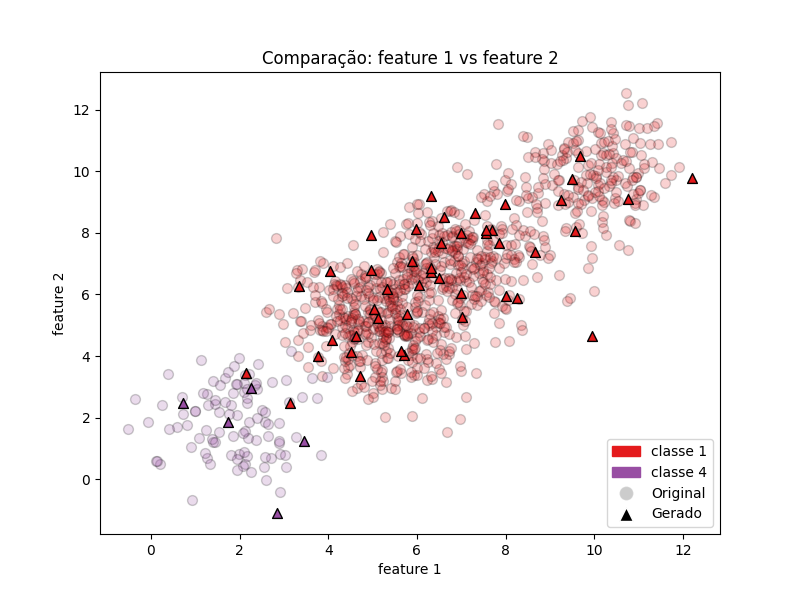
\includegraphics[width=\textwidth]{fig/q1_i6_x1x2.png}
            \caption{Feature 1 vs Feature 2}
            \label{fig:q1_i6_x1x2}
        \end{subfigure}
        \hfill
        \begin{subfigure}{0.45\textwidth}
            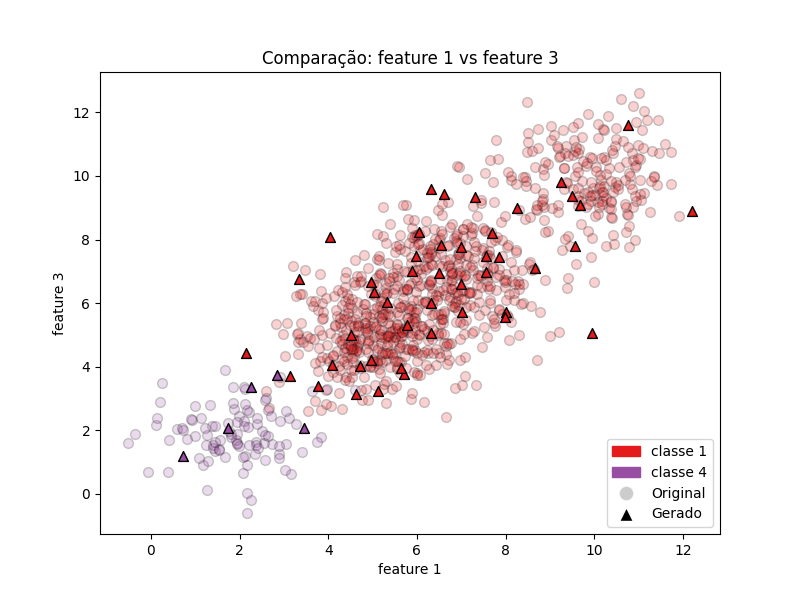
\includegraphics[width=\textwidth]{fig/q1_i6_x1x3.png}
            \caption{Feature 1 vs Feature 3}
            \label{fig:q1_i6_x1x3}
        \end{subfigure}
        
        \vspace{0.5cm}
        
        \begin{subfigure}{0.45\textwidth}
            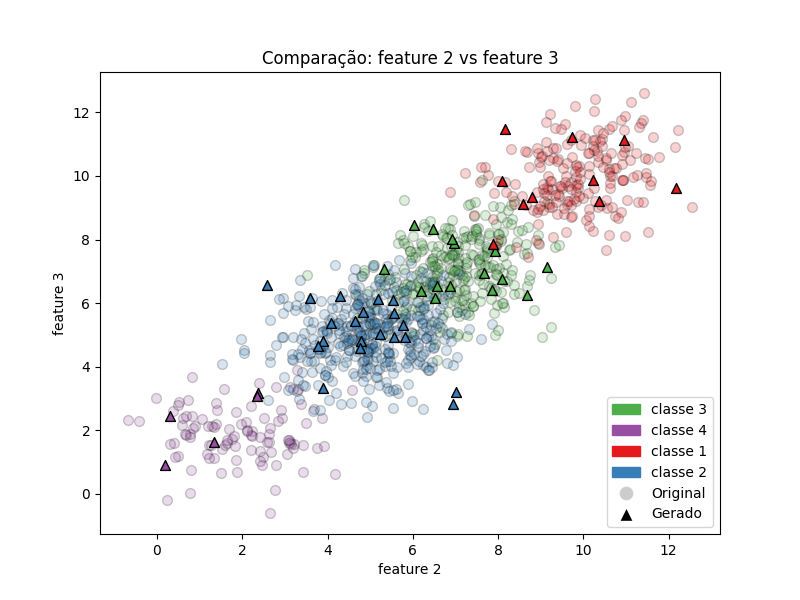
\includegraphics[width=\textwidth]{fig/q1_i6_x2x3.png}
            \caption{Feature 2 vs Feature 3}
            \label{fig:q1_i6_x2x3}
        \end{subfigure}
        \hfill
        \begin{subfigure}{0.45\textwidth}
            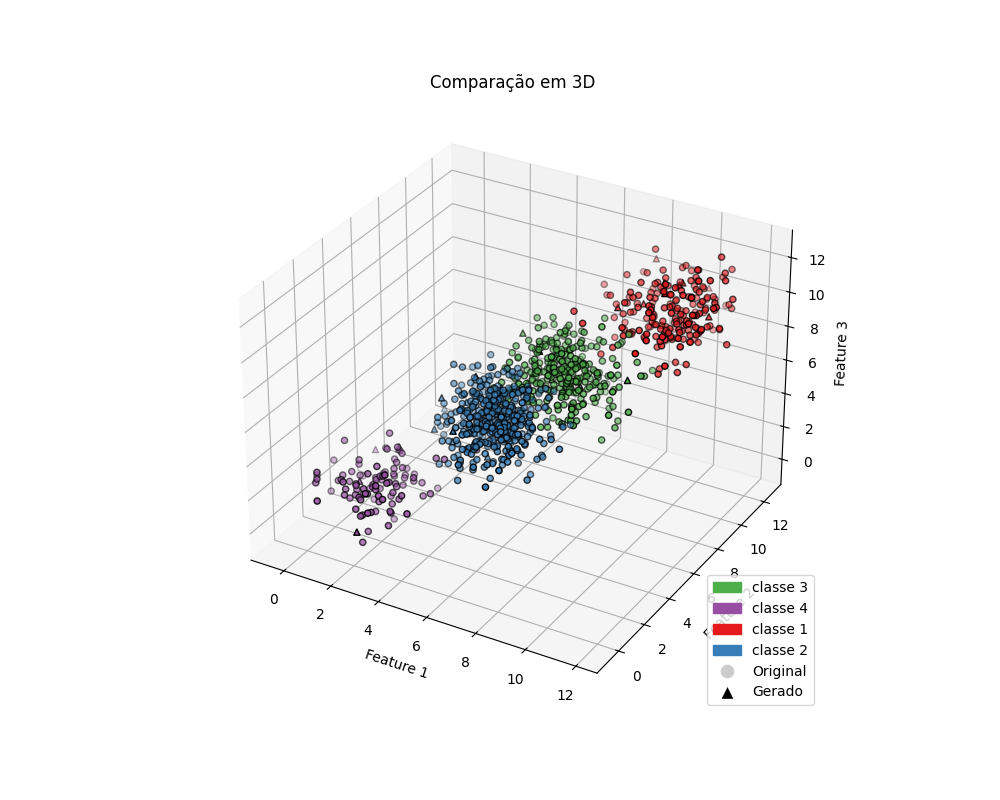
\includegraphics[width=\textwidth]{fig/q1_i6_3d.png}
            \caption{Gráfico 3D das features}
            \label{fig:q1_i6_3d}
        \end{subfigure}
        
        \caption{Visualização dos dados em 2D e 3D}
        \label{fig:q1_i6_combined}
    \end{figure}
\end{enumerate}
